\section{Discrete Fourier Transform and Fast Fourier Transform Theory}

\subsection{Discrete Fourier Transform (DFT)}

The Discrete Fourier Transform (DFT) is a fundamental tool in digital signal processing that maps a finite-length discrete-time signal from the time domain into the frequency domain. Given a discrete-time sequence $x(n)$ of length $N$, the DFT is defined as \cite{proakis_dsp}:

\begin{equation}
X(k) = \sum_{n=0}^{N-1} x(n) W_N^{nk}, \quad k = 0,1,\dots,N-1
\end{equation}

where the complex exponential term
\begin{equation}
W_N^{nk} = e^{-j\frac{2\pi nk}{N}} = \cos\left(\frac{2\pi nk}{N}\right) - j\sin\left(\frac{2\pi nk}{N}\right)
\end{equation}
is referred to as the \textit{twiddle factor}. In this formulation, $x(n)$ denotes the input sequence in the time domain, while $X(k)$ represents the discrete frequency-domain spectrum.

\subsection{Computational Complexity of DFT}

A direct implementation of the DFT requires $N$ complex multiplications and $(N-1)$ complex additions for each output sample $X(k)$. Consequently, the total arithmetic complexity of the DFT is given by:
\begin{itemize}
    \item Complex multiplications: $N^2$
    \item Complex additions: $N(N-1)$
\end{itemize}

Thus, the computational complexity of the DFT scales as:
\begin{equation}
\mathcal{O}(N^2)
\end{equation}

For large transform sizes (e.g., $N = 1024, 2048,$ or $4096$), this quadratic growth renders direct DFT computation impractical for real-time and hardware-based implementations.

\section{Fast Fourier Transform (FFT): Theory and Radix-2 DIT/DIF Algorithms}

\subsection{The idea of FFT}

Given a length-$N$ discrete-time sequence $x(n)$, the $N$-point Discrete Fourier Transform (DFT) is
\begin{equation}
X(k) = \sum_{n=0}^{N-1} x(n)\,W_N^{nk}, \quad k=0,1,\dots,N-1,
\label{eq:dft_def}
\end{equation}
where the twiddle factor is
\begin{equation}
W_N \triangleq e^{-j\frac{2\pi}{N}}, \qquad W_N^{nk}=e^{-j\frac{2\pi}{N}nk}.
\label{eq:twiddle_def}
\end{equation}

A direct evaluation of \eqref{eq:dft_def} is expensive because each output $X(k)$ requires $N$ complex multiplications and $(N-1)$ complex additions, resulting in $\mathcal{O}(N^2)$ arithmetic cost.

\textbf{The FFT idea} is to exploit the structure of the twiddle factors (periodicity and symmetry) and apply a \emph{divide-and-conquer} factorization: an $N$-point DFT is decomposed into multiple smaller DFTs (typically of size $N/2$), which are then combined with simple linear operations (``butterflies''). Repeating this decomposition recursively reduces the total complexity to $\mathcal{O}(N\log_2 N)$ for $N=2^m$.

\subsection{Radix-2 Building Block: 2-Point DFT and Butterfly}

The recursion of radix-2 FFT terminates at the 2-point DFT. For two samples $a$ and $b$, the 2-point DFT is
\begin{equation}
\begin{aligned}
A(0) &= a + b,\\
A(1) &= a - b.
\end{aligned}
\label{eq:2pt_dft}
\end{equation}

In FFT flow graphs, the \emph{butterfly} combines two complex inputs into two complex outputs using one twiddle multiplication and two additions/subtractions. A generic radix-2 butterfly can be written as
\begin{equation}
\begin{cases}
y_0 = a + b\cdot W,\\
y_1 = a - b\cdot W,
\end{cases}
\label{eq:butterfly_generic}
\end{equation}
where $W$ is an appropriate twiddle factor for that stage and branch. This operation is the fundamental computation repeated throughout FFT algorithms.

\subsection{Radix-2 DIT-FFT (Decimation-in-Time)}

\subsubsection{DIT Derivation (Time-Index Decomposition)}

Starting from \eqref{eq:dft_def}, split the time index $n$ into even and odd samples:
\[
x_e(r)\triangleq x(2r), \qquad x_o(r)\triangleq x(2r+1), \qquad r=0,1,\dots,\frac{N}{2}-1.
\]
Then,
\begin{align}
X(k)
&= \sum_{n=0}^{N-1} x(n) W_N^{nk} \nonumber\\
&= \sum_{r=0}^{\frac{N}{2}-1} x(2r) W_N^{(2r)k} + \sum_{r=0}^{\frac{N}{2}-1} x(2r+1) W_N^{(2r+1)k}.
\label{eq:dit_split1}
\end{align}
Using $W_N^{2rk}=W_{N/2}^{rk}$ and factoring out $W_N^k$ from the odd part yields
\begin{equation}
X(k) = E(k) + W_N^k\,O(k),
\label{eq:dit_Xk_firsthalf}
\end{equation}
where
\begin{equation}
E(k)\triangleq \sum_{r=0}^{\frac{N}{2}-1} x_e(r)\,W_{N/2}^{rk},\qquad
O(k)\triangleq \sum_{r=0}^{\frac{N}{2}-1} x_o(r)\,W_{N/2}^{rk}.
\label{eq:E_O_def}
\end{equation}
Here, $E(k)$ and $O(k)$ are \emph{$(N/2)$-point DFTs} of the even and odd subsequences. They are naturally defined for
\[
k = 0,1,\dots,\frac{N}{2}-1.
\]
To obtain the remaining $N/2$ outputs, use periodicity:
\begin{equation}
X\!\left(k+\frac{N}{2}\right) = E(k) - W_N^k\,O(k),
\qquad k=0,1,\dots,\frac{N}{2}-1.
\label{eq:dit_Xk_secondhalf}
\end{equation}

\paragraph{Meaning of terms (DIT).}
\begin{itemize}
    \item $E(k)$: spectrum computed from even-indexed time samples.
    \item $O(k)$: spectrum computed from odd-indexed time samples.
    \item $W_N^k$: phase-rotation factor that maps the odd-subsequence spectrum onto the full $N$-point frequency grid.
\end{itemize}
Although the intermediate spectra $E(k)$ and $O(k)$ are computed only for $k=0,\dots,N/2-1$, the pair \eqref{eq:dit_Xk_firsthalf}--\eqref{eq:dit_Xk_secondhalf} generates the full set of $N$ outputs $X(k)$ for $k=0,\dots,N-1$.

\subsubsection{The operation of DIT (Recursive Computation Down to 2 Points)}

Equations \eqref{eq:E_O_def} show that computing $X(k)$ reduces to computing two $(N/2)$-point DFTs. The same decomposition is applied recursively to $E(k)$ and $O(k)$:
\[
N \rightarrow \frac{N}{2} \rightarrow \frac{N}{4} \rightarrow \dots \rightarrow 2.
\]
At the final recursion level, every 2-point DFT is computed via \eqref{eq:2pt_dft}, and then results are combined stage-by-stage using butterfly relations \eqref{eq:dit_Xk_firsthalf}--\eqref{eq:dit_Xk_secondhalf}.

\paragraph{Ordering property (DIT).}
The DIT flow graph is typically arranged such that the \textbf{input is in bit-reversed order} and the \textbf{output is in natural order}. (Equivalently, one may keep natural-order input and perform an explicit bit-reversal permutation before processing.)

\begin{figure}[htbp]
    \centering
    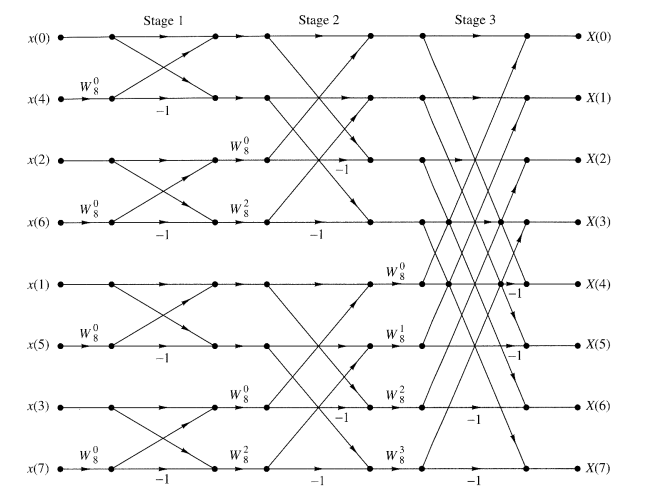
\includegraphics[width=0.95\linewidth]{images/fft_dit_8point.png}
    \caption{Radix-2 Decimation-in-Time (DIT) FFT flow graph for an 8-point DFT}
    \label{fig:fft_dit_8point}
\end{figure}

\subsubsection{Example: 8-Point Radix-2 DIT FFT}

An example of an 8-point radix-2 DIT FFT is illustrated in Fig.~\ref{fig:fft_dit_8point}. 
As discussed in the DIT formulation, the algorithm begins by decimating the input sequence in the time domain into even- and odd-indexed samples.

For $N=8$, the input sequence
\[
\{x(0),x(1),\dots,x(7)\}
\]
is decomposed into
\[
\text{Even-indexed samples: } \{x(0),x(2),x(4),x(6)\},
\]
\[
\text{Odd-indexed samples: } \{x(1),x(3),x(5),x(7)\}.
\]

As shown in Fig.~\ref{fig:fft_dit_8point}, the computation proceeds through three stages:
\begin{itemize}
    \item \textbf{Stage 1:} Four radix-2 butterflies combine pairs of samples that are $N/2 = 4$ indices apart, which means we have 4 2-point DFT in this stage. This stage corresponds to the first level of time-domain decimation.
    \item \textbf{Stage 2:} Two 4-point sub-FFTs are formed. Twiddle factors such as $W_8^0$ and $W_8^2$ appear on the branches, as indicated in the flow graph.
    \item \textbf{Stage 3:} The final stage combines the two 4-point spectra into the complete 8-point DFT using twiddle factors $W_8^k$, $k=0,1,2,3$.
\end{itemize}

Each butterfly shown in Fig.~\ref{fig:fft_dit_8point} performs one complex multiplication by a twiddle factor and two complex additions. The flow graph clearly visualizes the recursive nature of the DIT FFT, where smaller DFTs are computed first and then combined to produce the full spectrum.

\subsection{Radix-2 DIF-FFT (Decimation-in-Frequency)}

\subsubsection{DIF Derivation (Frequency-Index Decomposition)}

In DIF, we start by pairing time samples that are $N/2$ apart and form sums/differences first. Split the DFT sum into two halves:
\begin{align}
X(k)
&= \sum_{n=0}^{\frac{N}{2}-1} x(n) W_N^{nk}
 + \sum_{n=\frac{N}{2}}^{N-1} x(n) W_N^{nk}.
\end{align}
Let $n = r + N/2$ in the second sum:
\begin{align}
X(k)
&= \sum_{r=0}^{\frac{N}{2}-1} x(r) W_N^{rk}
 + \sum_{r=0}^{\frac{N}{2}-1} x\!\left(r+\frac{N}{2}\right) W_N^{(r+N/2)k} \nonumber\\
&= \sum_{r=0}^{\frac{N}{2}-1} \Big[x(r) + x\!\left(r+\frac{N}{2}\right)W_N^{(N/2)k}\Big] W_N^{rk}.
\label{eq:dif_mid1}
\end{align}
Using the identity $W_N^{(N/2)k} = e^{-j\pi k} = (-1)^k$, DIF separates the computation for even and odd $k$:

\paragraph{Even $k=2m$:}
\begin{align}
X(2m)
&= \sum_{r=0}^{\frac{N}{2}-1} \Big[x(r) + x\!\left(r+\frac{N}{2}\right)\Big] W_N^{r(2m)} \nonumber\\
&= \sum_{r=0}^{\frac{N}{2}-1} a(r)\, W_{N/2}^{rm},
\label{eq:dif_even}
\end{align}
where
\begin{equation}
a(r)\triangleq x(r)+x\!\left(r+\frac{N}{2}\right).
\label{eq:a_def}
\end{equation}

\paragraph{Odd $k=2m+1$:}
\begin{align}
X(2m+1)
&= \sum_{r=0}^{\frac{N}{2}-1} \Big[x(r) - x\!\left(r+\frac{N}{2}\right)\Big] W_N^{r(2m+1)} \nonumber\\
&= \sum_{r=0}^{\frac{N}{2}-1} \Big[x(r) - x\!\left(r+\frac{N}{2}\right)\Big] W_N^{r}\, W_{N/2}^{rm} \nonumber\\
&= \sum_{r=0}^{\frac{N}{2}-1} b(r)\, W_{N/2}^{rm},
\label{eq:dif_odd}
\end{align}
where
\begin{equation}
b(r)\triangleq \Big[x(r)-x\!\left(r+\frac{N}{2}\right)\Big]\,W_N^{r}.
\label{eq:b_def}
\end{equation}

Equations \eqref{eq:dif_even}--\eqref{eq:dif_odd} show that:
\begin{itemize}
    \item The \textbf{even-indexed outputs} $\{X(0),X(2),\dots,X(N-2)\}$ are obtained by an $(N/2)$-point DFT of $a(r)$.
    \item The \textbf{odd-indexed outputs} $\{X(1),X(3),\dots,X(N-1)\}$ are obtained by an $(N/2)$-point DFT of $b(r)$.
\end{itemize}

\subsubsection{DIF Butterfly and Its Meaning}

The DIF butterfly operates on paired inputs $x(r)$ and $x(r+N/2)$:
\begin{equation}
\begin{cases}
u(r) = x(r) + x(r+N/2),\\
v(r) = \big(x(r) - x(r+N/2)\big)\,W_N^{r},
\end{cases}
\quad r=0,1,\dots,\frac{N}{2}-1.
\label{eq:dif_butterfly}
\end{equation}

\paragraph{Meaning of terms (DIF).}
\begin{itemize}
    \item The sum $u(r)$ forms the input of the sub-DFT that produces the \emph{even} frequency bins.
    \item The difference $(x(r)-x(r+N/2))$ captures the complementary component needed for \emph{odd} bins, and multiplying by $W_N^{r}$ applies the required phase rotation.
    \item After this first butterfly stage, the problem decomposes into two independent $(N/2)$-point DFTs (one for even bins, one for odd bins).
\end{itemize}

\subsubsection{The operation of DIF (Recursive Computation Down to 2 Points)}

DIF recursion follows:
\[
N \rightarrow \frac{N}{2} \rightarrow \frac{N}{4} \rightarrow \dots \rightarrow 2,
\]
but the key difference from DIT is \textbf{where} the twiddle multiplication occurs:
\begin{itemize}
    \item DIF performs \textbf{add/sub first}, then multiplies the \textbf{difference branch} by a twiddle factor (see \eqref{eq:dif_butterfly}).
    \item The resulting sequences are then transformed by smaller DFTs (recursively), until the base 2-point DFT \eqref{eq:2pt_dft}.
\end{itemize}

\paragraph{Ordering property (DIF).}
DIF is commonly arranged so that the \textbf{input is in natural order} and the \textbf{output is in bit-reversed order}. (Equivalently, one may compute in natural order and then apply a bit-reversal permutation at the output.)

\begin{figure}[htbp]
    \centering
    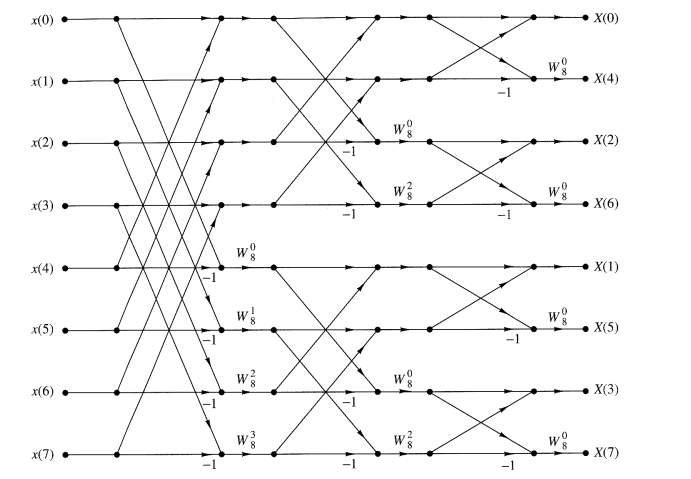
\includegraphics[width=0.95\linewidth]{images/fft_dif_8point.png}
    \caption{Radix-2 Decimation-in-Frequency (DIF) FFT flow graph for an 8-point DFT}
    \label{fig:fft_dif_8point}
\end{figure}

\subsubsection{Example: 8-Point Radix-2 DIT FFT}

An example of an 8-point radix-2 DIT FFT is illustrated in Fig.~\ref{fig:fft_dit_8point}. 
As discussed in the DIT formulation, the algorithm begins by decimating the input sequence in the time domain into even- and odd-indexed samples.

For $N=8$, the input sequence
\[
\{x(0),x(1),\dots,x(7)\}
\]
is decomposed into
\[
\text{Even-indexed samples: } \{x(0),x(2),x(4),x(6)\},
\]
\[
\text{Odd-indexed samples: } \{x(1),x(3),x(5),x(7)\}.
\]

As shown in Fig.~\ref{fig:fft_dit_8point}, the computation proceeds through three stages:
\begin{itemize}
    \item \textbf{Stage 1:} Four radix-2 butterflies combine pairs of samples that are $N/2 = 4$ indices apart. This stage corresponds to the first level of time-domain decimation.
    \item \textbf{Stage 2:} Two 4-point sub-FFTs are formed. Twiddle factors such as $W_8^0$ and $W_8^2$ appear on the branches, as indicated in the flow graph.
    \item \textbf{Stage 3:} The final stage combines the two 4-point spectra into the complete 8-point DFT using twiddle factors $W_8^k$, $k=0,1,2,3$.
\end{itemize}

Each butterfly shown in Fig.~\ref{fig:fft_dit_8point} performs one complex multiplication by a twiddle factor and two complex additions. The flow graph clearly visualizes the recursive nature of the DIT FFT, where smaller DFTs are computed first and then combined to produce the full spectrum.

\subsection{DIT vs. DIF: Two Implementations of the Same FFT}

DIT and DIF are \textbf{two algorithmic realizations} of the FFT principle:
\begin{itemize}
    \item Both compute the same DFT values $X(k)$.
    \item Both reduce the DFT into smaller transforms until reaching 2-point DFTs.
    \item The difference is the \textbf{decomposition viewpoint} and \textbf{twiddle placement}:
    \begin{itemize}
        \item DIT: decimate in \emph{time}, twiddle multiplication appears in the combination of sub-DFTs.
        \item DIF: decimate in \emph{frequency}, twiddle multiplication appears after forming sums/differences.
    \end{itemize}
\end{itemize}
Hence, the main purpose is identical: replace one long $N$-term summation by a structured computation built from many small butterflies, then combine the partial results to obtain the full spectrum.

\subsection{Computational Complexity of Radix-2 FFT (from Butterfly Counting)}

A radix-2 FFT with $N=2^m$ has $\log_2 N$ stages. At each stage:
\begin{itemize}
    \item The data are processed by $\frac{N}{2}$ butterflies (each butterfly consumes two inputs).
    \item Each butterfly performs \textbf{one complex multiplication} (by a twiddle factor) and \textbf{two complex additions} (one sum and one difference).
\end{itemize}

Therefore, the total arithmetic counts are:
\begin{align}
\text{Complex multiplications} \quad &=
\left(\frac{N}{2}\right)\log_2 N,
\label{eq:fft_cmuls}\\
\text{Complex additions} \quad &=
N\log_2 N.
\label{eq:fft_cadds}
\end{align}

This directly implies the overall FFT complexity:
\begin{equation}
\mathcal{O}(N\log_2 N),
\end{equation}
which is dramatically smaller than the direct DFT complexity $\mathcal{O}(N^2)$. The butterfly-based reasoning above matches the standard interpretation shown in the provided textbook excerpt (each stage uses $N/2$ butterflies, total stages $\log_2 N$) and is consistent with hardware-oriented FFT literature.


